% Standalone source for the paper figure; build with figures/build.sh
\documentclass[border=1pt]{standalone}
% Shared preamble for the standalone figure sources.
\usepackage{times}
\usepackage{amsmath,amssymb}
\usepackage{xcolor}
\usepackage{textcomp}
\usepackage{tikz}
\usepackage{pgfplots}
\usetikzlibrary{arrows.meta,positioning,calc,fit,backgrounds}
\usepgfplotslibrary{fillbetween}
\pgfplotsset{compat=1.16}

% Colours are colour-blind safe (Okabe--Ito) and every figure also separates
% its classes by line style or fill, so the figures stay readable in greyscale.
\definecolor{cObs}{HTML}{0072B2}   % observed by the network
\definecolor{cHid}{HTML}{D55E00}   % hidden / unexplained
\definecolor{cHelp}{HTML}{009E73}  % safety helpers
\definecolor{cInk}{HTML}{333333}

\tikzset{
  box/.style={draw=cInk!70, rounded corners=1.5pt, fill=white, align=center,
              font=\scriptsize, inner sep=3pt, minimum height=0.8cm,
              line width=0.5pt},
  obs/.style={box, draw=cObs, fill=cObs!8},
  hid/.style={box, draw=cHid, fill=cHid!10},
  help/.style={box, draw=cHelp, fill=cHelp!10},
  flow/.style={-{Stealth[length=4pt]}, line width=0.6pt, draw=cInk!80},
  lbl/.style={font=\scriptsize, text=cInk!85, inner sep=1.5pt, align=center},
}
\pgfplotsset{
  every axis/.append style={font=\scriptsize, tick label style={font=\scriptsize},
                            label style={font=\scriptsize},
                            title style={font=\scriptsize\bfseries}, line width=0.5pt},
}

\begin{document}
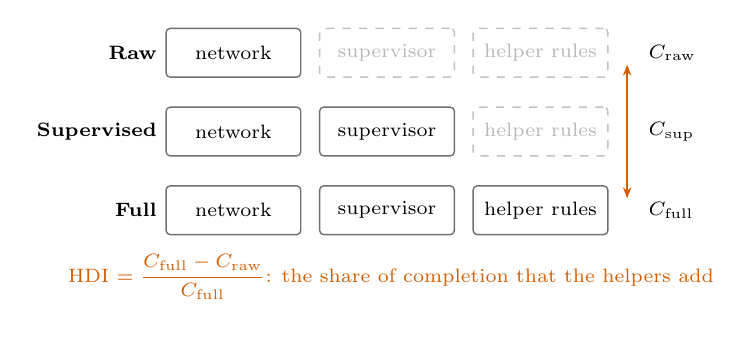
\begin{tikzpicture}[x=1cm,y=1cm]
\tikzset{chip/.style={box, text width=1.5cm, minimum height=0.62cm},
         off/.style={chip, draw=cInk!30, text=cInk!35, fill=none, dashed}}
\node[anchor=east, font=\scriptsize\bfseries] at (1.35,1.0) {Raw};
\node[anchor=east, font=\scriptsize\bfseries] at (1.35,0.0) {Supervised};
\node[anchor=east, font=\scriptsize\bfseries] at (1.35,-1.0) {Full};
% Raw
\node[obs, chip] at (2.2,1.0) {network};
\node[off] at (4.15,1.0) {supervisor};
\node[off] at (6.1,1.0) {helper rules};
% Supervised
\node[obs, chip] at (2.2,0.0) {network};
\node[help, chip] at (4.15,0.0) {supervisor};
\node[off] at (6.1,0.0) {helper rules};
% Full
\node[obs, chip] at (2.2,-1.0) {network};
\node[help, chip] at (4.15,-1.0) {supervisor};
\node[help, chip] at (6.1,-1.0) {helper rules};
% completion labels
\node[anchor=west, font=\scriptsize] at (7.35,1.0) {$C_{\text{raw}}$};
\node[anchor=west, font=\scriptsize] at (7.35,0.0) {$C_{\text{sup}}$};
\node[anchor=west, font=\scriptsize] at (7.35,-1.0) {$C_{\text{full}}$};
\draw[{Stealth[length=4pt]}-{Stealth[length=4pt]}, line width=0.6pt, draw=cHid]
  (7.2,0.85) -- (7.2,-0.85);
\node[align=center, font=\scriptsize, text=cHid] at (4.2,-1.85)
  {HDI $=\dfrac{C_{\text{full}}-C_{\text{raw}}}{C_{\text{full}}}$:
   the share of completion that the helpers add};
\end{tikzpicture}
\end{document}
